\section{Module B: the plant-hydraulic failure engine}\label{sec:B}

Module B is the part of the framework that has to be right where the data run out. It is therefore kept as simple as the physiology allows, fully transparent, and tested against closed-form solutions. It does not simulate a tree; it tracks the one state variable that decides survival in a drought, the water stored between stomatal closure and lethal xylem embolism.

\subsection{Vulnerability, closure and the lethal threshold}
The xylem vulnerability curve is the logistic form \citep{Pammenter1998}
\begin{equation}\label{eq:plc}
\PLC(\psi)=\frac{100}{1+\exp[a\,(\psi-P_{50})]},\qquad a=\frac{S}{25},
\end{equation}
where $S$ (\% MPa$^{-1}$) is the slope at $P_{50}$, since $|d\PLC/d\psi|_{P_{50}}=25a$. Inverting, the water potential at a given loss $L$ is $\psi_L=P_{50}+a^{-1}\ln\!\big[(100-L)/L\big]$, so that $P_{88}=P_{50}-a^{-1}\ln(88/12)$. Death is set at $L=88$ for angiosperms \citep{Urli2013} and $L=50$ for conifers \citep{Brodribb2009}, giving the lethal potential $\psi_{\text{crit}}=\psi_L$. Stomata close as the predawn water potential falls, $f_{gs}(\psi)=[1+\exp\{a_s(\psi-\psi_{gs50})\}]^{-1}$, and we take $\psi_{\text{close}}=\psi_{gs90}=\psi_{gs50}-a_s^{-1}\ln 9$ as the potential at which they are effectively shut.

\subsection{Two phases of survival}
\textbf{Phase 1, time to closure,} is delivered by Module A: stomata are treated as closed on day $d$ when the root-zone potential satisfies $\psi_{s,d}\le\psi_{\text{close}}$. Because this phase carries most of the survival time \citep{Waite2026,Gauthey2026}, the accuracy of $\psi_s$, and hence of soil depth, rooting depth and PET, matters more for timing than any trait in phase 2. This is the reason Module A is validated first.

\textbf{Phase 2, time to critical failure,} starts at closure. With stomata shut, the plant loses water only through the cuticle and bark, and draws on its stored water. A mass balance per unit leaf area gives
\begin{equation}\label{eq:massbal}
C\,\frac{d\psi}{dt}=-E_{\min},\qquad E_{\min}=g_{\min}(T)\,\frac{\VPD_{24}}{P_{\text{atm}}},\qquad B=C\,(\psi_{\text{close}}-\psi_{\text{crit}}),\qquad t_{\text{crit}}=\frac{B}{E_{\min}},
\end{equation}
with $C$ the effective whole-plant capacitance (mmol\,m$^{-2}$\,MPa$^{-1}$), $g_{\min}$ in mmol\,m$^{-2}$\,s$^{-1}$, $\VPD_{24}/P_{\text{atm}}$ dimensionless (mol\,mol$^{-1}$), and $B$ the hydraulic buffer between closure and death ($t_{\text{crit}}$ is in seconds, divided by 86\,400 for days below). The closed form \citep[cf.][]{MartinStPaul2017} is the unit test for the daily engine, which accumulates the index
\begin{equation}\label{eq:hfi}
A_d=(1-\rho\,\ind[\text{open}_d])\,A_{d-1}+\ind[\text{closed}_d]\cdot86400\,E_{\min,d},\qquad \HFI_d=A_d/B,
\end{equation}
where $\rho\in[0,1]$ is the fraction of the deficit refilled on a day when stomata are open (rain, or ${\psi_s>\psi_{\text{close}}}$). Hydraulic failure is defined as $\max_d\HFI_d\ge1$ within a year.

\textbf{The heat phase transition.} Residual conductance is not constant: it increases slowly with temperature, then abruptly above a critical temperature $T_p$ at which the cuticle loses its barrier properties \citep{Cochard2019,Duursma2019},
\begin{equation}\label{eq:gmin}
g_{\min}(T)=\begin{cases}g_{25}\,Q_a^{(T-25)/10}, & T\le T_p,\\[2pt] g_{25}\,Q_a^{(T_p-25)/10}\,Q_b^{(T-T_p)/10}, & T>T_p,\end{cases}
\end{equation}
with $Q_a\approx1.2$ and $Q_b\approx4.8$ of the order reported by \citet{Cochard2019}, and $g_{25}$, $T_p$ species-level random variables ($T_p$ spans roughly 30--45\,$^\circ$C across species). A worked example with the placeholder trait set of the skeleton ($C=3\times10^4$, $P_{50}=-3$~MPa, $S=40$, $\psi_{\text{close}}=-2.5$~MPa, $g_{25}=3$, $T_p=38\,^\circ$C, angiosperm): $\psi_{\text{crit}}=-4.25$~MPa, $B=5.2\times10^4$~mmol\,m$^{-2}$, and at $\VPD_{24}=2$~kPa, $P_{\text{atm}}=90$~kPa, $t_{\text{crit}}$ is 8.3 days at 30\,$^\circ$C but 2.8 days at 44\,$^\circ$C. Same tree, same VPD, 14~K hotter, a third of the time; the difference is the phase transition, and it is exactly what a model trained only on the current climate cannot see (Fig.~\ref{fig:hyd}b). Trait values in the figure and skeleton are placeholders that exercise the code and are not results.

\begin{figure}[t]
\centering
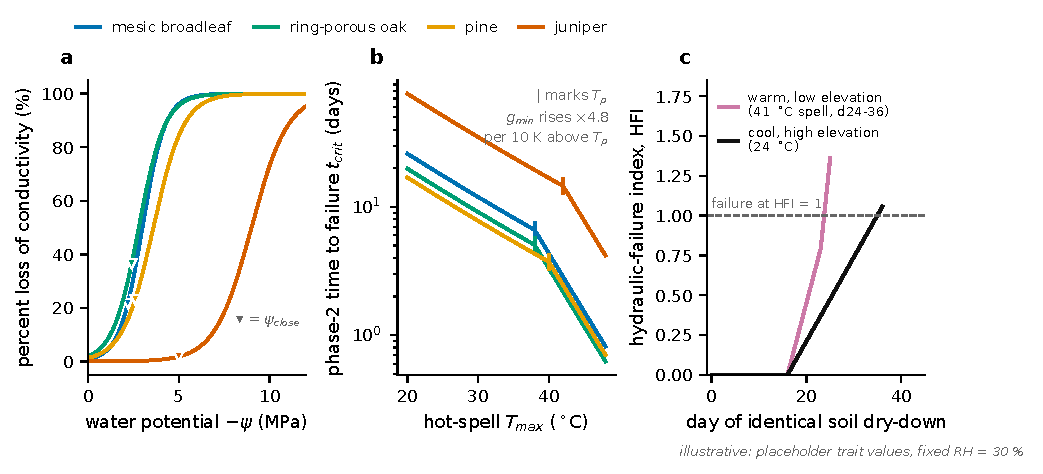
\includegraphics[width=\linewidth]{fig3_hydraulics.pdf}
\caption{The hydraulic engine, with illustrative placeholder traits for four functional groups. (a)~Vulnerability curves; triangles mark the stomatal-closure potential. (b)~Phase-2 time to failure against hot-spell temperature at fixed relative humidity; $g_{\min}$ steepens the fall above each group's $T_p$ (tick). (c)~The same soil dry-down at a warm low site with a 41\,$^\circ$C spell and at a cool high site: closure occurs on the same day, failure much earlier at the warm site.}\label{fig:hyd}
\end{figure}

\subsection{From traits to a probability}
Trait values differ among individuals and are uncertain to us; the two must not be mixed. We therefore sample in two levels. An outer loop of 50 draws takes hyper-parameters (group means and spreads of $P_{50}$, $S$, $\psi_{\text{close}}$, $C$, $g_{25}$, $T_p$) from posteriors built on XFT, TRY and the $g_{\min}$ compilation and updated with local measurements; an inner loop of 200 draws samples individuals. The mechanistic annual hazard is the share of individuals that fail,
\begin{equation}\label{eq:hmech}
\hmech_{iky}=\frac1M\sum_{m=1}^{M}\ind\Big[\max_{d\in y}\HFI^{(m)}_{iky,d}\ge1\Big],
\end{equation}
and the spread of $\hmech$ across the outer loop is its knowledge uncertainty. Seedlings, established saplings and mature trees form separate trait classes because capacitance per unit leaf area, rooting depth and $\psi_{\text{close}}$ change with ontogeny, and because larger trees are more exposed to drought \citep{Bennett2015}.

\textbf{Emulation.} Running the engine for every 30~m cell, year and draw is not feasible, so we emulate it. A Latin hypercube over stress-spell summaries (longest closed spell, mean $\VPD_{24}$ and $T$ during it, number of closed days) and trait-group descriptors is passed through the full engine, and a gradient-boosting regressor with monotone constraints (increasing in spell length, VPD and temperature; decreasing in $C$ and $B$) is fitted to $\hmech$. Monotonicity is guaranteed by construction, and the emulator must reproduce the full engine on a held-out hypercube to within 0.02 in absolute hazard before it is used.

\subsection{Pattern-oriented calibration, and what Module B does not claim}\label{sec:pom}
Prior trait draws are constrained by the patterns that Armenia already exhibits, using approximate Bayesian computation \citep{Grimm2005,Beaumont2010}. A draw $\theta$ is run over 2000--2024 forcing at reference sites and accepted if its summary statistics fall within a tolerance of the observed ones: (i) the Boyce index of predicted viability against present-day adult occurrence for each group; (ii) rank correlation between engine-predicted failure years and tree-ring growth collapses at the chronology sites \citep{Voss2025,Stepanyan2026,OpalaOwczarek2021}; (iii) observed dieback frequency by elevation band; and (iv) published orderings from dry-down experiments \citep{Waite2026}. The posterior narrows the priors; whatever mismatch remains is absorbed by a two-parameter recalibration on the link scale, $\cloglog(\tilde h^{\text{mech}})=a_g+b_g\,\cloglog(\hmech)$ with $b_g>0$, fitted per functional group on the observed event panel with hierarchical shrinkage. A monotone map of the link cannot change the shape of the physical response, so extrapolation keeps its mechanistic form.

The engine assumes constant capacitance, a plant hydraulically isolated from the soil once stomata close, no explicit carbon-starvation pathway, leaf temperature equal to $T_{\max}$ (tested against a leaf--air offset), and a single hydraulic threshold per group. Each is a documented limitation and a sensitivity experiment; none is hidden in the code.
